\chapter{ऑक्सीकरण और अपचयन}\label{ch:g11:redox}

जस्ते की एक पट्टी कॉपर सल्फ़ेट के नीले विलयन में डुबोई जाती है। कुछ ही मिनटों में
उसकी सतह एक स्पंजी, लाल-भूरी परत के नीचे काली पड़ जाती है; एक घंटे बाद
विलयन का नीला रंग फीका पड़ चुका होता है। जहाँ पहले कुछ नहीं था, वहाँ ताँबा \omterm{def:g9:periodic-table-first-look:metal}{धातु}
प्रकट हो गई है, और जस्ता अदृश्य \omterm{def:g9:ions:ion}{आयनों} के रूप में विलयन में चला गया है।
कुछ भी गरम नहीं किया गया, कोई गैस नहीं निकली, ऑक्सीजन ने कोई भाग नहीं लिया ---
फिर भी रसायनज्ञ इसे \omterm{def:g11:redox:oxidation}{ऑक्सीकरण} कहते हैं। कभी इस शब्द का अर्थ था ``ऑक्सीजन से
संयोग करना''; अब इसका अर्थ कुछ अधिक व्यापक और अधिक उपयोगी है:
\omterm{def:g9:inside-the-atom:nucleus}{इलेक्ट्रॉनों} का खोना। यह अध्याय \omterm{def:g9:inside-the-atom:nucleus}{इलेक्ट्रॉनों} का पीछा करता है।

\begin{recall}
\omterm{def:g9:ions:ion}{आयन} वह \omterm{def:g7:atoms-and-molecules:atom}{परमाणु} या \omterm{def:g7:atoms-and-molecules:atom}{परमाणुओं} का समूह है जिसने \omterm{def:g9:inside-the-atom:nucleus}{इलेक्ट्रॉन} ग्रहण किए हैं या खोए हैं
(\cref{ch:g9:ions})। लोहा या जस्ता जैसी \omterm{def:g9:periodic-table-first-look:metal}{धातु}
हाइड्रोक्लोरिक अम्ल से अभिक्रिया करके हाइड्रोजन और \omterm{def:g9:periodic-table-first-look:metal}{धातु} \omterm{def:g9:ions:ion}{आयन} देती है
(\cref{ch:g9:metals-acids-corrosion})। \omterm{def:g10:the-mole:amount}{मोल} में \omterm{def:g10:the-mole:amount}{पदार्थ की मात्रा} $n$
द्रव्यमान $m$ से $n = m/M$ द्वारा निकाली जाती है
(\cref{ch:g10:the-mole})।
\end{recall}

\begin{omfigure}
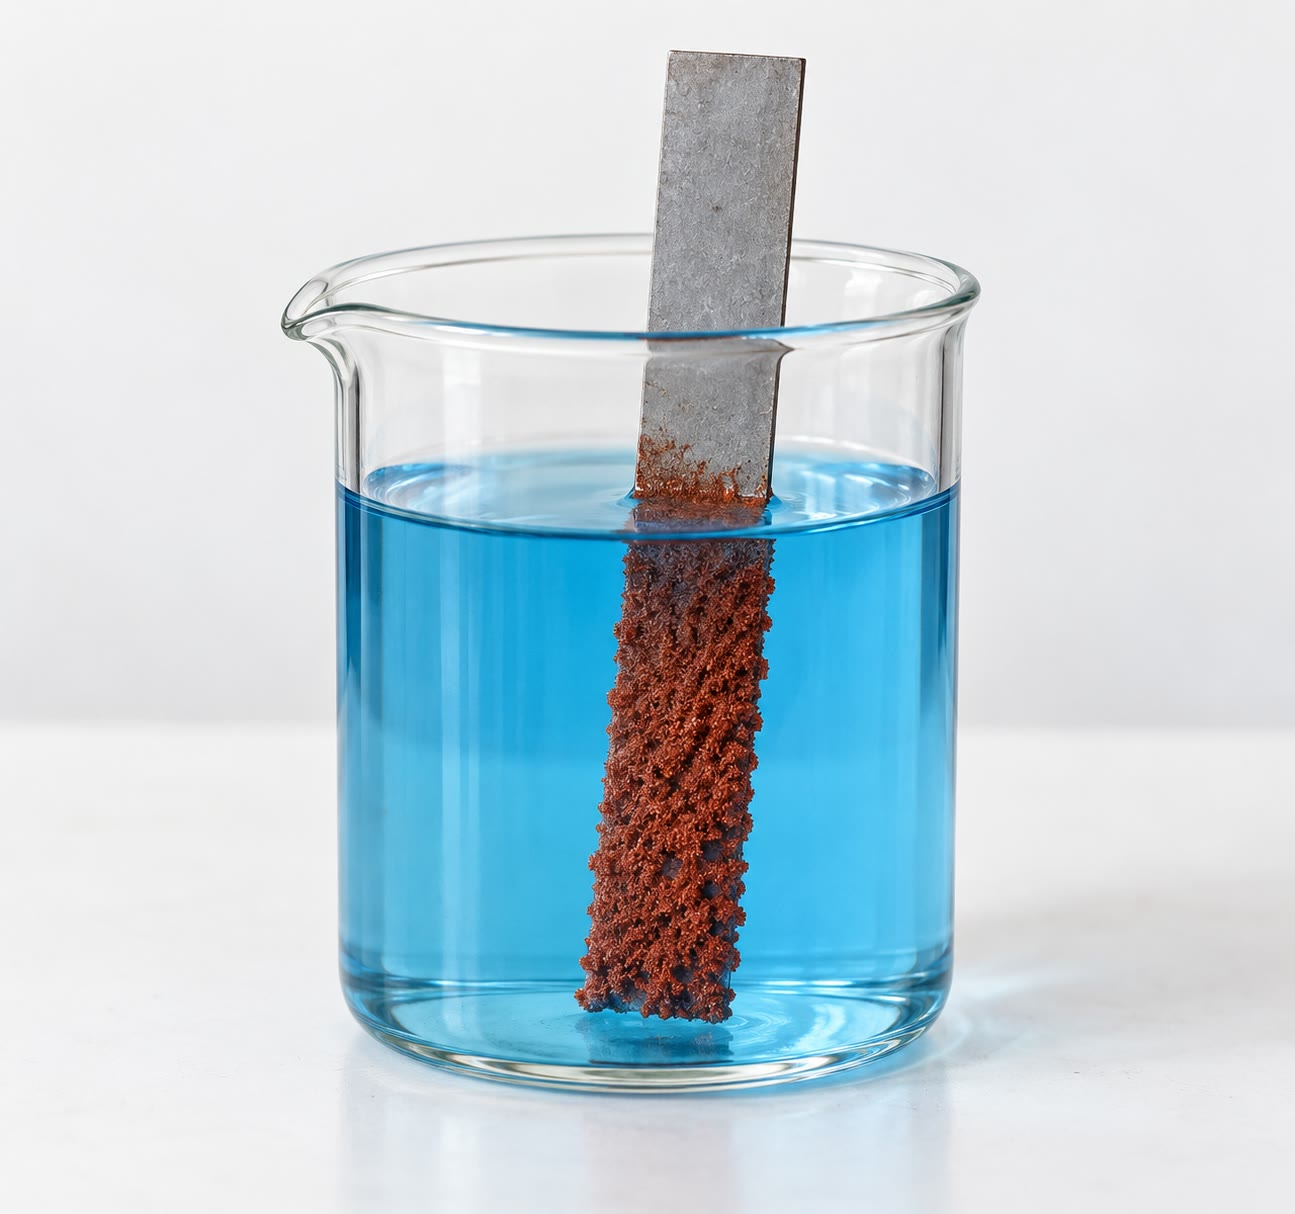
\includegraphics[width=0.55\linewidth]{images/book1/ai/g11-zinc-copper-sulfate.jpg}

{\small कॉपर सल्फ़ेट विलयन में जस्ते की एक पट्टी: जस्ते पर ताँबा जमता है,
और जस्ता \omterm{def:g9:ions:ion}{आयन} विलयन में उसकी जगह ले लेते हैं।}
\end{omfigure}

\section{ऑक्सीकारक और अपचायक}

\begin{definition}[ऑक्सीकारक और अपचायक]\label{def:g11:redox:oxidant}
\emph{ऑक्सीकारक}\index{ऑक्सीकारक} वह स्पीशीज़ है जो एक या अधिक \omterm{def:g9:inside-the-atom:nucleus}{इलेक्ट्रॉन}
ग्रहण कर सकती है। \emph{अपचायक}\index{अपचायक} वह स्पीशीज़ है जो एक या
अधिक \omterm{def:g9:inside-the-atom:nucleus}{इलेक्ट्रॉन} दे सकती है।
\end{definition}

\begin{definition}[ऑक्सीकरण और अपचयन]\label{def:g11:redox:oxidation}
\emph{ऑक्सीकरण}\index{ऑक्सीकरण} \omterm{def:g9:inside-the-atom:nucleus}{इलेक्ट्रॉनों} का खोना है;
\emph{अपचयन}\index{अपचयन} \omterm{def:g9:inside-the-atom:nucleus}{इलेक्ट्रॉनों} का ग्रहण है। \omterm{def:g11:redox:oxidant}{अपचायक}
ऑक्सीकृत होता है; \omterm{def:g11:redox:oxidant}{ऑक्सीकारक} अपचयित होता है।
\end{definition}

\begin{remark}[याद रखने का एक तरीका]\label{rem:g11:redox:remember}
\emph{\omterm{def:g11:redox:oxidation}{अपचयन}} में स्पीशीज़ का आवेश घटता है: दो \omterm{def:g9:inside-the-atom:nucleus}{इलेक्ट्रॉन} ग्रहण करने वाला \ce{Cu^{2+}}
\ce{Cu} बन जाता है, आवेश $+2 \to 0$। \omterm{def:g11:redox:oxidation}{ऑक्सीकरण} में
आवेश बढ़ता है: \ce{Zn -> Zn^{2+} + 2e-}, $0 \to +2$।
\end{remark}

\begin{definition}[अपचयोपचय युग्म और अर्ध-समीकरण]\label{def:g11:redox:couple}
एक \omterm{def:g11:redox:oxidant}{ऑक्सीकारक} और वह \omterm{def:g11:redox:oxidant}{अपचायक} जो वह \omterm{def:g9:inside-the-atom:nucleus}{इलेक्ट्रॉन} ग्रहण करके बनता है, मिलकर एक
\emph{अपचयोपचय युग्म}\index{अपचयोपचय युग्म} बनाते हैं, जिसे \omterm{def:g11:redox:oxidant}{ऑक्सीकारक}
पहले रखकर ऑक्स/अप लिखा जाता है: \ce{Cu^{2+}}/\ce{Cu}, \ce{Zn^{2+}}/\ce{Zn}। किसी युग्म
के भीतर \omterm{def:g9:inside-the-atom:nucleus}{इलेक्ट्रॉनों} के आदान-प्रदान का वर्णन उसका
\emph{अर्ध-समीकरण}\index{अर्ध-समीकरण} करता है,
\[
  \text{ऑक्स} + n\,\ce{e-} \ce{<=>} \text{अप}, % ce-unbalanced-ok (generic form)
\]
जो \omterm{def:g7:atoms-and-molecules:atom}{परमाणुओं} और आवेश दोनों में संतुलित होता है, उदाहरण के लिए
$\ce{Cu^{2+}(aq) + 2e- <=> Cu(s)}$। दोहरा तीर बताता है कि
आदान-प्रदान किसी भी दिशा में हो सकता है।
\end{definition}

\begin{example}[धातुएँ और उनके आयन]\label{ex:g11:redox:metals}
हर \omterm{def:g9:periodic-table-first-look:metal}{धातु} अपने \omterm{def:g9:ions:ion}{आयन} के साथ एक युग्म बनाती है:
\begin{center}
\begin{tabular}{ll}
\hline
युग्म & \omterm{def:g11:redox:couple}{अर्ध-समीकरण} \\
\hline
\ce{Ag+}/\ce{Ag} & \ce{Ag+ + e- <=> Ag} \\
\ce{Cu^{2+}}/\ce{Cu} & \ce{Cu^{2+} + 2e- <=> Cu} \\
\ce{Fe^{2+}}/\ce{Fe} & \ce{Fe^{2+} + 2e- <=> Fe} \\
\ce{Zn^{2+}}/\ce{Zn} & \ce{Zn^{2+} + 2e- <=> Zn} \\
\ce{Al^{3+}}/\ce{Al} & \ce{Al^{3+} + 3e- <=> Al} \\
\hline
\end{tabular}
\end{center}
\omterm{def:g9:ions:ion}{आयन} भी युग्म बना सकते हैं: युग्म \ce{Fe^{3+} + e- <=> Fe^{2+}} के लिए
\ce{Fe^{3+}}/\ce{Fe^{2+}}, और \ce{I2 + 2e- <=> 2I-} के लिए
\ce{I2}/\ce{I-}। हाइड्रोजन भी: \ce{2H+ + 2e- <=> H2} के लिए
\ce{H+}/\ce{H2}।
\end{example}

\begin{remark}[एक स्पीशीज़, दो भूमिकाएँ]\label{rem:g11:redox:amphoteric}
कोई स्पीशीज़ एक युग्म का \omterm{def:g11:redox:oxidant}{अपचायक} और दूसरे युग्म का \omterm{def:g11:redox:oxidant}{ऑक्सीकारक} हो सकती है।
\omterm{def:g9:ions:ion}{आयन} \ce{Fe^{2+}} युग्म \ce{Fe^{2+}}/\ce{Fe} का \omterm{def:g11:redox:oxidant}{ऑक्सीकारक} है और
\ce{Fe^{3+}}/\ce{Fe^{2+}} का \omterm{def:g11:redox:oxidant}{अपचायक}। वह कौन-सी भूमिका निभाता है, यह
अभिक्रिया में उसके साथी पर निर्भर करता है।
\end{remark}

\section{अपचयोपचय अभिक्रियाएँ}

\begin{definition}[अपचयोपचय अभिक्रिया]\label{def:g11:redox:reaction}
\emph{अपचयोपचय अभिक्रिया}\index{अपचयोपचय अभिक्रिया} एक युग्म के \omterm{def:g11:redox:oxidant}{अपचायक} से
दूसरे युग्म के \omterm{def:g11:redox:oxidant}{ऑक्सीकारक} तक \omterm{def:g9:inside-the-atom:nucleus}{इलेक्ट्रॉनों} का स्थानांतरण है।
\omterm{def:g11:redox:oxidant}{अपचायक} ऑक्सीकृत होता है और \omterm{def:g11:redox:oxidant}{ऑक्सीकारक} अपचयित, एक ही समय पर।
\end{definition}

\begin{proposition}[कोई मुक्त इलेक्ट्रॉन नहीं]\label{prop:g11:redox:no-free-electrons}
विलयन में \omterm{def:g9:inside-the-atom:nucleus}{इलेक्ट्रॉन} मुक्त रूप में नहीं रहते: \omterm{def:g11:redox:oxidant}{अपचायक} द्वारा दिया गया हर
\omterm{def:g9:inside-the-atom:nucleus}{इलेक्ट्रॉन} \omterm{def:g11:redox:oxidant}{ऑक्सीकारक} ले लेता है। इसलिए \omterm{def:g11:redox:reaction}{अपचयोपचय अभिक्रिया} का समीकरण
दोनों \omterm{def:g11:redox:couple}{अर्ध-समीकरणों} को जोड़कर मिलता है, हर एक को उस संख्या से गुणा करके
जो दिए गए \omterm{def:g9:inside-the-atom:nucleus}{इलेक्ट्रॉनों} को लिए गए \omterm{def:g9:inside-the-atom:nucleus}{इलेक्ट्रॉनों} के बराबर कर दे;
तब \omterm{def:g9:inside-the-atom:nucleus}{इलेक्ट्रॉन} कट जाते हैं और समीकरण में दिखाई नहीं देते।
\end{proposition}

\begin{example}[जस्ता और कॉपर आयन]\label{ex:g11:redox:zinc-copper}
आरंभिक दृश्य में जस्ता ऑक्सीकृत होता है और कॉपर \omterm{def:g9:ions:ion}{आयन}
अपचयित होते हैं:
\[
\begin{array}{l@{\qquad}l}
  \ce{Zn(s) -> Zn^{2+}(aq) + 2e-} & \text{(ऑक्सीकरण)}\\
  \ce{Cu^{2+}(aq) + 2e- -> Cu(s)} & \text{(अपचयन)}\\
  \hline
  \ce{Zn(s) + Cu^{2+}(aq) -> Zn^{2+}(aq) + Cu(s)} &
\end{array}
\]
हर जस्ता \omterm{def:g7:atoms-and-molecules:atom}{परमाणु} से दो \omterm{def:g9:inside-the-atom:nucleus}{इलेक्ट्रॉन} एक कॉपर \omterm{def:g9:ions:ion}{आयन} तक जाते हैं। विलयन का नीला
रंग \ce{Cu^{2+}} \omterm{def:g9:ions:ion}{आयनों} का रंग है; जैसे-जैसे वे खपते हैं, वह फीका पड़ता है,
जबकि रंगहीन \ce{Zn^{2+}} \omterm{def:g9:ions:ion}{आयन} उनकी
जगह ले लेते हैं।
\end{example}

\begin{omfigure}
\begin{tikzpicture}[font=\small, >=Stealth,
    ion/.style={circle, draw=black!70, minimum size=10mm, inner sep=0pt}]
  % the zinc strip and the solution
  \fill[black!18] (0,0) rectangle (1.6,4);
  \draw[black!60] (1.6,0) -- (1.6,4);
  \node[anchor=south] at (0.8,0.08) {जस्ता};
  \fill[omWater!60] (1.6,0) rectangle (9.0,4);
  \node[anchor=north east] at (8.95,3.95) {विलयन};
  % a zinc atom leaves as an ion
  \node[ion, fill=black!30] (zn) at (1.15,3.0) {\ce{Zn}};
  \node[ion, fill=white] (znion) at (5.0,3.0) {\ce{Zn^{2+}}};
  \draw[->, thick, omProp] (zn.east) -- (znion.west)
    node[midway, above] {ऑक्सीकरण};
  % the electrons travel through the metal
  \draw[->, thick, omDef, dashed] (0.75,2.45) -- (0.75,1.55)
    node[midway, right] {2\,\ce{e-}};
  % a copper ion is reduced on the surface
  \node[ion, fill=omDef!35] (cuion) at (5.0,1.0) {\ce{Cu^{2+}}};
  \node[ion, fill=orange!55!brown] (cu) at (2.12,1.0) {\ce{Cu}};
  \draw[->, thick, omProp] (cuion.west) -- (cu.east)
    node[midway, above] {अपचयन};
  \node[anchor=west, align=left] at (6.1,2.0) {हर जस्ता परमाणु\\ एक कॉपर आयन को\\ दो इलेक्ट्रॉन देता है};
\end{tikzpicture}

{\small जस्ते की सतह पर। एक जस्ता \omterm{def:g7:atoms-and-molecules:atom}{परमाणु} दो \omterm{def:g9:inside-the-atom:nucleus}{इलेक्ट्रॉन} खोता है और
\ce{Zn^{2+}} \omterm{def:g9:ions:ion}{आयन} के रूप में चला जाता है; दोनों \omterm{def:g9:inside-the-atom:nucleus}{इलेक्ट्रॉन} \omterm{def:g9:periodic-table-first-look:metal}{धातु} से होकर
सतह को छूते एक \ce{Cu^{2+}} \omterm{def:g9:ions:ion}{आयन} तक पहुँचते हैं, जो ताँबे का \omterm{def:g7:atoms-and-molecules:atom}{परमाणु} बन जाता है
और पट्टी पर ही रह जाता है।}
\end{omfigure}

\begin{omfigure}
\begin{tikzpicture}[font=\small]
  \pic at (0,0) {beaker={0.75}{omDef!45}};
  \fill[black!35] (-0.15,0.25) rectangle (0.15,2.5);
  \draw[black!65] (-0.15,0.25) rectangle (0.15,2.5);
  \node[anchor=north, align=center] at (0,-0.15) {शुरुआत में:\\ नीला \ce{Cu^{2+}} विलयन};
  \draw[->, thick, omProp] (1.3,1) -- (3.2,1) node[midway, above] {एक घंटा};
  \pic at (4.5,0) {beaker={0.75}{omDef!12}};
  \fill[black!35] (4.35,0.25) rectangle (4.65,2.5);
  \fill[orange!55!brown] (4.3,0.25) rectangle (4.7,1.5);
  \draw[black!65] (4.35,0.25) rectangle (4.65,2.5);
  \node[anchor=north, align=center] at (4.5,-0.15) {बाद में: फीका विलयन,\\ जस्ते पर ताँबा};
\end{tikzpicture}

{\small क्या दिखता है: पट्टी के डूबे भाग पर ताँबे का जमाव, और
\ce{Cu^{2+}} \omterm{def:g9:ions:ion}{आयनों} के नीले रंग का फीका पड़ना।}
\end{omfigure}

\begin{example}[अम्ल में धातुएँ, फिर से]\label{ex:g11:redox:acid}
जब लोहा हाइड्रोक्लोरिक अम्ल में \omterm{def:g2:mixing-and-dissolving:dissolve}{घुलता} है, तो लोहा ऑक्सीकृत होता है और
\ce{H+} \omterm{def:g9:ions:ion}{आयन} हाइड्रोजन में अपचयित होते हैं:
\[
  \ce{Fe(s) + 2H+(aq) -> Fe^{2+}(aq) + H2(g)}.
\]
युग्म \ce{Fe^{2+}}/\ce{Fe} और \ce{H+}/\ce{H2} हैं; क्लोराइड
\omterm{def:g9:ions:ion}{आयन} कोई भाग नहीं लेते।
\end{example}

\begin{inthelab}[चाँदी का पेड़]
साफ़ ताँबे के तार का एक कुंडल तनु सिल्वर नाइट्रेट विलयन,
\ce{Ag+(aq) + NO3^-(aq)}, के बीकर में लटकाया जाता है। एक घंटे के भीतर
चमकीली चाँदी की शाखित सुइयाँ तार के साथ उग आती हैं, और रंगहीन विलयन
हल्का नीला हो जाता है: \ce{Cu(s) + 2Ag+(aq) -> Cu^{2+}(aq) + 2Ag(s)}। यह
प्रयोग शिक्षक दस्ताने और चश्मा पहनकर करते हैं, और बाद में
विलयन को ख़तरनाक अपशिष्ट के रूप में एकत्र किया जाता है।
\end{inthelab}

\begin{safety}{\ghs[0.82cm]{GHS03}\ghs[0.82cm]{GHS05}\ghs[0.82cm]{GHS08}\ghs[0.82cm]{GHS09}}
% ledger: ghs:AgNO3
सिल्वर नाइट्रेट: एक \omterm{def:g11:redox:oxidant}{ऑक्सीकारक} जो आग को बढ़ा सकता है (GHS03); त्वचा और आँखों के
लिए संक्षारक, और यह त्वचा पर काले धब्बे छोड़ता है (GHS05); स्वास्थ्य के लिए ख़तरा
(GHS08); जलीय जीवन के लिए अत्यंत विषैला, इसलिए यह कभी सिंक में नहीं बहाया जाता
(GHS09)।
\end{safety}

\begin{omfigure}
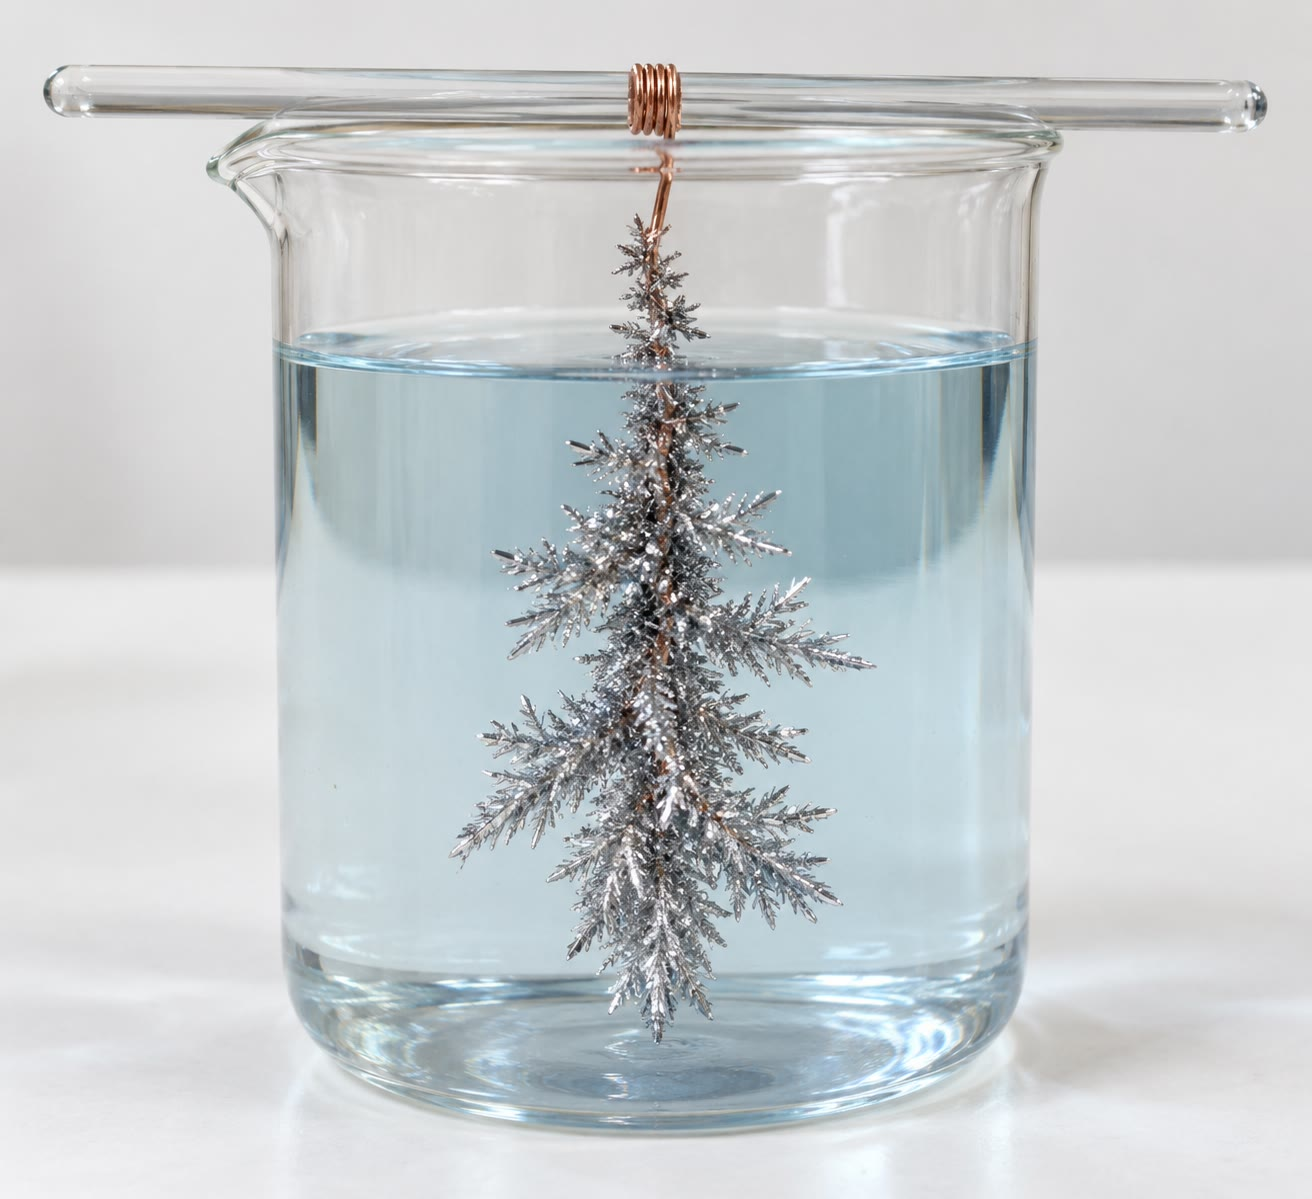
\includegraphics[width=0.5\linewidth]{images/book1/ai/g11-silver-tree.jpg}

{\small सिल्वर नाइट्रेट विलयन में ताँबे के तार पर उगते चाँदी के
क्रिस्टल।}
\end{omfigure}

\section{अर्ध-समीकरणों को संतुलित करना}

कई महत्त्वपूर्ण युग्मों में ऑक्सीजन होती है और वे \omterm{def:g9:acids-bases-ph:acidic}{अम्लीय विलयनों} के लिए
लिखे जाते हैं, जहाँ \ce{H+} \omterm{def:g9:ions:ion}{आयन} मौजूद होते हैं। उनके \omterm{def:g11:redox:couple}{अर्ध-समीकरणों} को संतुलित करने के लिए
पानी के \omterm{def:g7:atoms-and-molecules:molecule}{अणु} और \ce{H+} \omterm{def:g9:ions:ion}{आयन} चाहिए।

\begin{method}[अम्लीय विलयन में अर्ध-समीकरण संतुलित करना]\label{met:g11:redox:balance}
\omterm{def:g9:acids-bases-ph:acidic}{अम्लीय विलयन} में किसी युग्म ऑक्स/अप का \omterm{def:g11:redox:couple}{अर्ध-समीकरण} लिखने के लिए:
\begin{enumerate}
  \item ऑक्स को बाईं ओर और अप को दाईं ओर लिखिए, और उस \omterm{def:g7:atoms-and-molecules:atom}{परमाणु} को संतुलित कीजिए
        जो न O है न H;
  \item ऑक्सीजन \omterm{def:g7:atoms-and-molecules:atom}{परमाणुओं} को पानी के \omterm{def:g7:atoms-and-molecules:molecule}{अणुओं} \ce{H2O} से संतुलित कीजिए;
  \item हाइड्रोजन \omterm{def:g7:atoms-and-molecules:atom}{परमाणुओं} को \ce{H+} \omterm{def:g9:ions:ion}{आयनों} से संतुलित कीजिए;
  \item आवेश को \omterm{def:g9:inside-the-atom:nucleus}{इलेक्ट्रॉनों} \ce{e-} से, बाईं ओर, संतुलित कीजिए;
  \item जाँचिए: दोनों ओर हर \omterm{def:g7:atoms-and-molecules:atom}{परमाणु} की संख्या समान, कुल आवेश
        समान।
\end{enumerate}
\end{method}

\begin{example}[परमैंगनेट आयन]\label{ex:g11:redox:permanganate}
युग्म \ce{MnO4^-}/\ce{Mn^{2+}} (गहरे बैंगनी से लगभग
रंगहीन) के लिए: मैंगनीज़ संतुलित है; बाईं ओर के चार O दाईं ओर
$\ce{4H2O}$ देते हैं; उनके आठ H बाईं ओर $\ce{8H+}$ देते हैं; बाईं ओर
आवेश $-1 + 8 = +7$ है, दाईं ओर $+2$, इसलिए बाईं ओर पाँच
\omterm{def:g9:inside-the-atom:nucleus}{इलेक्ट्रॉन} जोड़े जाते हैं:
\[
  \ce{MnO4^-(aq) + 8H+(aq) + 5e- <=> Mn^{2+}(aq) + 4H2O(l)}.
\]
\end{example}

\begin{example}[डाइक्रोमेट आयन]\label{ex:g11:redox:dichromate}
\ce{Cr2O7^{2-}}/\ce{Cr^{3+}} (नारंगी से हरा) के लिए: दाईं ओर दो क्रोमियम;
सात O \ce{7H2O} देते हैं; चौदह H \ce{14H+} देते हैं; आवेश
बाईं ओर $-2 + 14 = +12$, दाईं ओर के $2 \times 3 = +6$ के मुक़ाबले, इसलिए
छह \omterm{def:g9:inside-the-atom:nucleus}{इलेक्ट्रॉन}:
\[
  \ce{Cr2O7^{2-}(aq) + 14H+(aq) + 6e- <=> 2Cr^{3+}(aq) + 7H2O(l)}.
\]
\end{example}

\begin{method}[अपचयोपचय समीकरण लिखना]\label{met:g11:redox:combine}
एक युग्म के \omterm{def:g11:redox:oxidant}{ऑक्सीकारक} ऑक्स$_1$ और दूसरे युग्म के \omterm{def:g11:redox:oxidant}{अपचायक}
अप$_2$ के बीच की अभिक्रिया का समीकरण लिखने के लिए:
\begin{enumerate}
  \item दोनों \omterm{def:g11:redox:couple}{अर्ध-समीकरण} लिखिए, पहला
        \omterm{def:g11:redox:oxidation}{अपचयन} की दिशा में (ऑक्स$_1 \to$ अप$_1$), दूसरा
        \omterm{def:g11:redox:oxidation}{ऑक्सीकरण} की दिशा में (अप$_2 \to$ ऑक्स$_2$);
  \item उन्हें उन सबसे छोटी संख्याओं से गुणा कीजिए जो \omterm{def:g9:inside-the-atom:nucleus}{इलेक्ट्रॉनों} को
        बराबर कर दें;
  \item उन्हें जोड़िए; \omterm{def:g9:inside-the-atom:nucleus}{इलेक्ट्रॉन} कट जाते हैं, और दोनों ओर दिखने वाले कुछ \ce{H+} और
        \ce{H2O} भी कट सकते हैं;
  \item \omterm{def:g7:atoms-and-molecules:atom}{परमाणुओं} और आवेश को एक बार फिर जाँचिए।
\end{enumerate}
\end{method}

\begin{example}[परमैंगनेट और आयरन(II)]\label{ex:g11:redox:mno4-fe}
परमैंगनेट \omterm{def:g9:ions:ion}{आयन} \ce{Fe^{2+}} \omterm{def:g9:ions:ion}{आयनों} को \ce{Fe^{3+}} में ऑक्सीकृत करता है:
\[
\begin{array}{l@{\qquad}l}
  \ce{MnO4^- + 8H+ + 5e- -> Mn^{2+} + 4H2O} & \times 1\\
  \ce{Fe^{2+} -> Fe^{3+} + e-} & \times 5\\
  \hline
  \ce{MnO4^- + 8H+ + 5Fe^{2+} -> Mn^{2+} + 5Fe^{3+} + 4H2O} &
\end{array}
\]
बाईं ओर आवेश: $-1 + 8 + 10 = +17$; दाईं ओर: $2 + 15 = +17$।
यह अभिक्रिया अगले अध्याय में आयरन(II) की मात्रा मापने के लिए
इस्तेमाल की जाती है।
\end{example}

\section{हमारे आसपास के ऑक्सीकारक और अपचायक}

\begin{proposition}[कुछ सामान्य ऑक्सीकारक और अपचायक]\label{prop:g11:redox:common}
निम्नलिखित स्पीशीज़ प्रयोगशाला में और रोज़मर्रा के जीवन में बार-बार
मिलती हैं:
\begin{center}
\small
\begin{tabular}{lll}
\hline
स्पीशीज़ & भूमिका & उसके युग्म का \omterm{def:g11:redox:couple}{अर्ध-समीकरण} \\
\hline
डाइऑक्सीजन \ce{O2} & \omterm{def:g11:redox:oxidant}{ऑक्सीकारक} & \ce{O2 + 4H+ + 4e- <=> 2H2O} \\
डाइक्लोरीन \ce{Cl2} & \omterm{def:g11:redox:oxidant}{ऑक्सीकारक} & \ce{Cl2 + 2e- <=> 2Cl-} \\
हाइपोक्लोराइट \ce{ClO-} (ब्लीच) & \omterm{def:g11:redox:oxidant}{ऑक्सीकारक} & \ce{2ClO- + 4H+ + 2e- <=> Cl2 + 2H2O} \\
हाइड्रोजन परॉक्साइड \ce{H2O2} & \omterm{def:g11:redox:oxidant}{ऑक्सीकारक} & \ce{H2O2 + 2H+ + 2e- <=> 2H2O} \\
परमैंगनेट \ce{MnO4^-} & \omterm{def:g11:redox:oxidant}{ऑक्सीकारक} & \ce{MnO4^- + 8H+ + 5e- <=> Mn^{2+} + 4H2O} \\
\omterm{def:g9:periodic-table-first-look:metal}{धातुएँ} \ce{M} (\ce{Fe}, \ce{Zn}, \ce{Al}\dots) & \omterm{def:g11:redox:oxidant}{अपचायक} & \ce{M^{n+} + $n$ e- <=> M} % ce-unbalanced-ok (generic)
\\
आयोडाइड \ce{I-} & \omterm{def:g11:redox:oxidant}{अपचायक} & \ce{I2 + 2e- <=> 2I-} \\
थायोसल्फ़ेट \ce{S2O3^{2-}} & \omterm{def:g11:redox:oxidant}{अपचायक} & \ce{S4O6^{2-} + 2e- <=> 2S2O3^{2-}} \\
ऐस्कॉर्बिक अम्ल \ce{C6H8O6} (विटामिन C) & \omterm{def:g11:redox:oxidant}{अपचायक} & \ce{C6H6O6 + 2H+ + 2e- <=> C6H8O6} \\
\hline
\end{tabular}
\end{center}
\end{proposition}

\begin{example}[ताँबा हरा हो जाता है]\label{ex:g11:redox:patina}
खुली \omterm{def:g4:air-a-mixture-of-gases:air}{हवा} में दशकों तक छोड़ी गई ताँबे की छतें और मूर्तियाँ धीरे-धीरे
हल्की हरी हो जाती हैं। \omterm{def:g4:air-a-mixture-of-gases:air}{वायु} की ऑक्सीजन ताँबे को \ce{Cu^{2+}} \omterm{def:g9:ions:ion}{आयनों} में ऑक्सीकृत करती है,
जो पानी और कार्बन डाइऑक्साइड के साथ एक पतली हरी परत, पैटिना, बनाते हैं।
लोहे पर \omterm{def:g9:metals-acids-corrosion:corrosion}{जंग} के विपरीत, पैटिना \omterm{def:g9:periodic-table-first-look:metal}{धातु} से चिपकी रहती है और
उसे आगे के क्षरण से बचाती है।
\end{example}

\begin{omfigure}
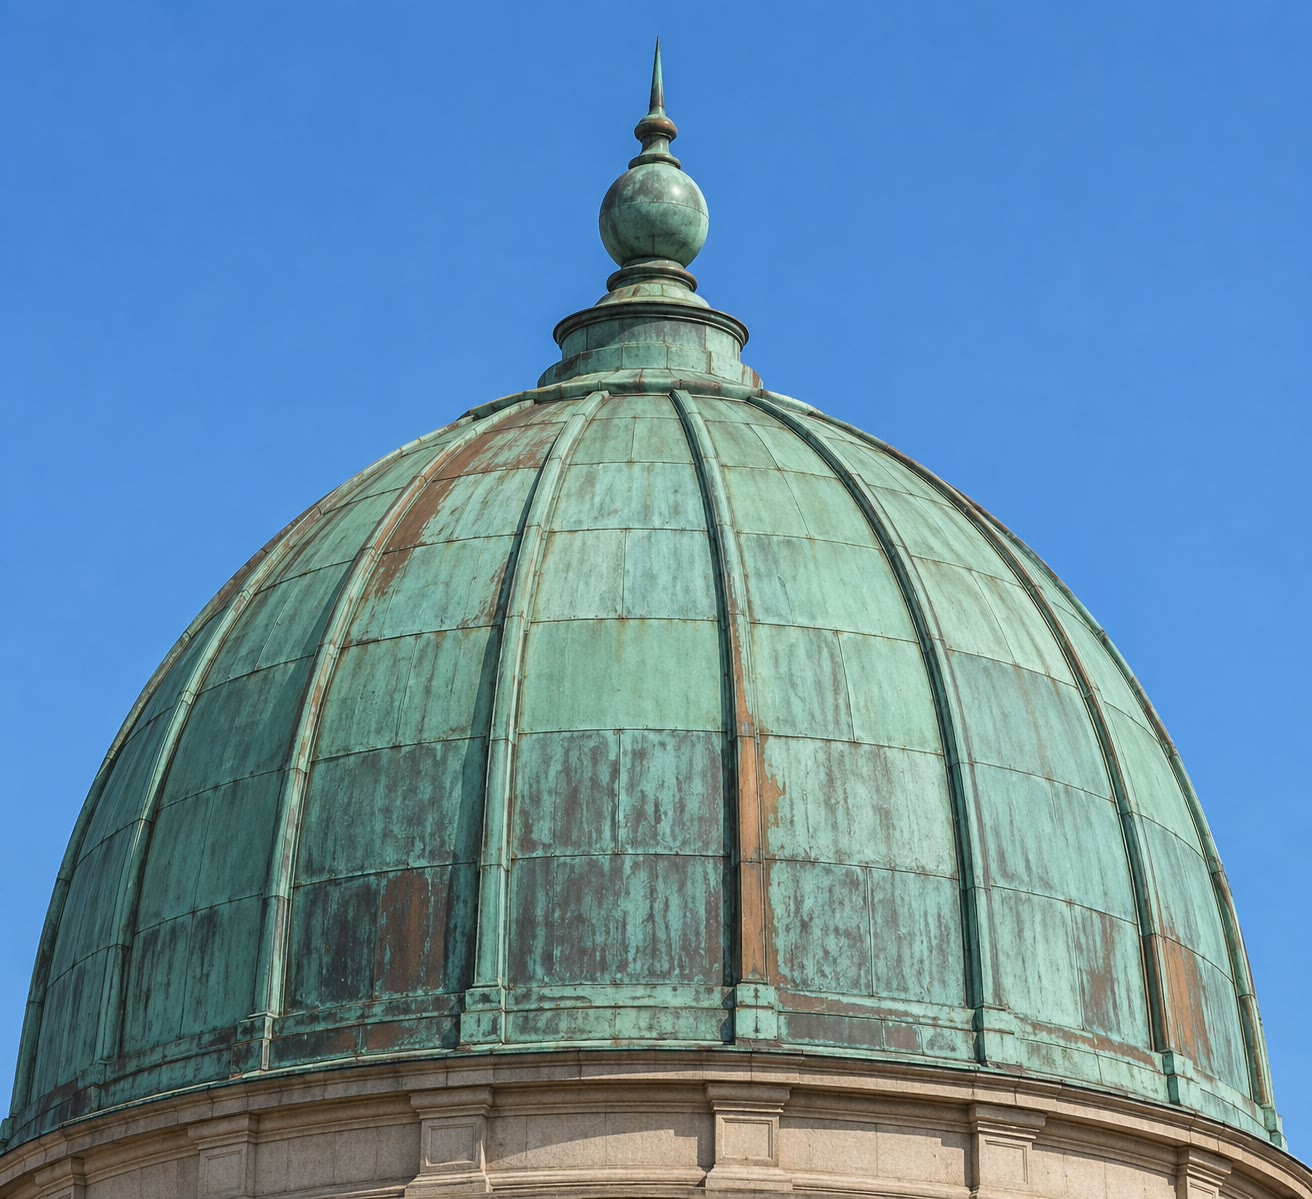
\includegraphics[width=0.48\linewidth]{images/book1/ai/g11-green-roof.jpg}

{\small दशकों तक \omterm{def:g4:air-a-mixture-of-gases:air}{हवा} में रहने के बाद ताँबे की एक छत: ऑक्सीकृत ताँबा एक
हरी पैटिना बनाता है।}
\end{omfigure}

\begin{remark}[प्रतिऑक्सीकारक]\label{rem:g11:redox:antioxidant}
भोजन में मिलाया गया ``प्रतिऑक्सीकारक'' एक \omterm{def:g11:redox:oxidant}{अपचायक} है जो भोजन से पहले
\omterm{def:g4:air-a-mixture-of-gases:air}{वायु} की ऑक्सीजन द्वारा ऑक्सीकृत हो जाता है। विटामिन C (ऐस्कॉर्बिक अम्ल) सबसे
आम है: नींबू का रस छिड़का गया कटा सेब कहीं अधिक धीरे भूरा होता है,
क्योंकि नींबू का विटामिन C पहले ऑक्सीकृत होता है।
\end{remark}

\section{अभ्यास}

\begin{exercise}[$\star$]\label{exo:g11:redox:1}
\omterm{def:g11:redox:oxidant}{ऑक्सीकारक}, \omterm{def:g11:redox:oxidant}{अपचायक}, \omterm{def:g11:redox:oxidation}{ऑक्सीकरण} और \omterm{def:g11:redox:oxidation}{अपचयन} की परिभाषा दीजिए।
\end{exercise}

\begin{exercise}[$\star$]\label{exo:g11:redox:2}
हर जोड़े के लिए \omterm{def:g11:redox:couple}{अपचयोपचय युग्म} ऑक्स/अप रूप में लिखिए: \ce{Fe} और
\ce{Fe^{2+}}; \ce{Ag} और \ce{Ag+}; \ce{I-} और \ce{I2}; \ce{Fe^{2+}}
और \ce{Fe^{3+}}।
\end{exercise}

\begin{exercise}[$\star$]\label{exo:g11:redox:3}
युग्मों \ce{Ag+}/\ce{Ag},
\ce{Al^{3+}}/\ce{Al}, \ce{Fe^{3+}}/\ce{Fe^{2+}} और \ce{Cl2}/\ce{Cl-} के \omterm{def:g11:redox:couple}{अर्ध-समीकरण} लिखिए।
\end{exercise}

\begin{exercise}[$\star$]\label{exo:g11:redox:4}
क्या रूपांतरण \ce{Fe -> Fe^{2+} + 2e-} \omterm{def:g11:redox:oxidation}{ऑक्सीकरण} है या
\omterm{def:g11:redox:oxidation}{अपचयन}? लोहा \omterm{def:g11:redox:oxidant}{ऑक्सीकारक} की तरह काम कर रहा है या \omterm{def:g11:redox:oxidant}{अपचायक} की तरह?
\end{exercise}

\begin{exercise}[$\star$]\label{exo:g11:redox:5}
अभिक्रिया \ce{Zn + Cu^{2+} -> Zn^{2+} + Cu} में ऑक्सीकृत स्पीशीज़,
अपचयित स्पीशीज़, \omterm{def:g11:redox:oxidant}{ऑक्सीकारक} और \omterm{def:g11:redox:oxidant}{अपचायक} के नाम बताइए, और
हर जस्ता \omterm{def:g7:atoms-and-molecules:atom}{परमाणु} के लिए स्थानांतरित \omterm{def:g9:inside-the-atom:nucleus}{इलेक्ट्रॉनों} की संख्या बताइए।
\end{exercise}

\begin{exercise}[$\star\star$]\label{exo:g11:redox:6}
\cref{met:g11:redox:balance} का चरण-दर-चरण पालन करते हुए, \omterm{def:g9:acids-bases-ph:acidic}{अम्लीय विलयन} में
युग्म \ce{H2O2}/\ce{H2O} का \omterm{def:g11:redox:couple}{अर्ध-समीकरण}
संतुलित कीजिए।
\end{exercise}

\begin{exercise}[$\star\star$]\label{exo:g11:redox:7}
आयोडीन \ce{I2} और
थायोसल्फ़ेट \omterm{def:g9:ions:ion}{आयन} \ce{S2O3^{2-}} के बीच की अभिक्रिया का समीकरण लिखिए, जो आयोडाइड \omterm{def:g9:ions:ion}{आयन} और
टेट्राथायोनेट \omterm{def:g9:ions:ion}{आयन} \ce{S4O6^{2-}} देती है।
\end{exercise}

\begin{exercise}[$\star\star$]\label{exo:g11:redox:8}
चाँदी के पेड़ वाली अभिक्रिया का समीकरण उसके दो
\omterm{def:g11:redox:couple}{अर्ध-समीकरणों} से लिखिए, और समझाइए कि विलयन नीला क्यों हो जाता है।
\end{exercise}

\begin{exercise}[$\star\star$]\label{exo:g11:redox:9}
विटामिन C, \ce{C6H8O6}, आयोडीन \ce{I2} से अभिक्रिया करता है। अभिक्रिया का
समीकरण लिखिए, और बताइए कि कौन-सी स्पीशीज़ \omterm{def:g11:redox:oxidant}{अपचायक} है।
\end{exercise}

\begin{exercise}[$\star\star$]\label{exo:g11:redox:10}
ऐलुमिनियम कॉपर(II) \omterm{def:g9:ions:ion}{आयनों} से अभिक्रिया करता है। समीकरण लिखिए, और समझाइए
कि \omterm{def:g11:redox:couple}{अर्ध-समीकरणों} को 2 से और 3 से गुणा क्यों करना पड़ता है।
\end{exercise}

\begin{exercise}[$\star\star$]\label{exo:g11:redox:11}
हाइड्रोजन परॉक्साइड \omterm{def:g9:acids-bases-ph:acidic}{अम्लीय विलयन} में आयरन(II) \omterm{def:g9:ions:ion}{आयनों} को आयरन(III) \omterm{def:g9:ions:ion}{आयनों} में
ऑक्सीकृत करता है। समीकरण लिखिए।
\end{exercise}

\begin{exercise}[$\star\star\star$]\label{exo:g11:redox:12}
कॉपर(II) \omterm{def:g9:ions:ion}{आयनों} की अधिकता वाले विलयन में जस्ते की एक पट्टी का द्रव्यमान \qty{1.30}{g}
घटता है। ताँबे का कितना द्रव्यमान जमता है? लीजिए
$M(\ce{Zn}) = \qty{65.4}{g/mol}$ और $M(\ce{Cu}) = \qty{63.5}{g/mol}$।
\end{exercise}

\begin{exercise}[$\star\star\star$]\label{exo:g11:redox:13}
\omterm{def:g9:acids-bases-ph:acidic}{अम्लीय विलयन} में डाइक्रोमेट \omterm{def:g9:ions:ion}{आयनों} द्वारा आयरन(II) \omterm{def:g9:ions:ion}{आयनों} के \omterm{def:g11:redox:oxidation}{ऑक्सीकरण} का
समीकरण लिखिए। डाइक्रोमेट \omterm{def:g9:ions:ion}{आयनों} के \qty{0.010}{mol} द्वारा \ce{Fe^{2+}} की कितनी मात्रा
ऑक्सीकृत होती है?
\end{exercise}

\begin{exercise}[$\star\star\star$]\label{exo:g11:redox:14}
ब्लीच में हाइपोक्लोराइट \omterm{def:g9:ions:ion}{आयन} \ce{ClO-} और क्लोराइड \omterm{def:g9:ions:ion}{आयन}
\ce{Cl-} होते हैं। युग्मों \ce{ClO-}/\ce{Cl2} और \ce{Cl2}/\ce{Cl-} का उपयोग करके
उस अभिक्रिया का समीकरण लिखिए जो ब्लीच के किसी अम्ल से मिलने पर होती है, और
समझाइए कि ब्लीच और अम्लीय डीस्केलिंग उत्पादों, दोनों के लेबल
उन्हें कभी न मिलाने की चेतावनी क्यों देते हैं।
\end{exercise}

\begin{exercise}[$\star\star\star$]\label{exo:g11:redox:15}
जस्ते की सतह वाले चित्र में \omterm{def:g9:inside-the-atom:nucleus}{इलेक्ट्रॉन} \omterm{def:g9:periodic-table-first-look:metal}{धातु} से होकर जाते हैं,
विलयन से होकर नहीं। \cref{prop:g11:redox:no-free-electrons} का उपयोग करके
समझाइए कि ताँबा स्वयं जस्ते की पट्टी पर ही क्यों जमता है, बीकर में
कहीं और क्यों नहीं।
\end{exercise}

\section{समस्या: साँस परीक्षण}

\begin{problem}[{सप्ताहांत समस्या --- साँस-ऐल्कोहॉल नली का
रसायन: दो युग्म, नारंगी से हरा रंग-परिवर्तन, एथेनॉल का वह द्रव्यमान
जिसे एक नली पकड़ सकती है, और वह ईंधन सेल जिसने उसकी जगह ली}]
\label{pb:g11:redox:1}
% ledger: ghs:K2Cr2O7, breath:ratio; molar masses from tools/molar_mass.py
% (0.1-rounded weights): K2Cr2O7 294.2, C2H6O 46.0 g/mol
पहले साँस-ऐल्कोहॉल परीक्षणों में काँच की एक नली इस्तेमाल होती थी जो अम्ल में
नारंगी पोटैशियम डाइक्रोमेट, \ce{K2Cr2O7}, से लेपित सिलिका के दानों से भरी होती थी।
नली से फूँकी गई साँस का एथेनॉल, \ce{CH3CH2OH},
डाइक्रोमेट \omterm{def:g9:ions:ion}{आयनों} को हरे \ce{Cr^{3+}} \omterm{def:g9:ions:ion}{आयनों} में अपचयित करता है और स्वयं एथेनोइक
अम्ल, \ce{CH3COOH}, में ऑक्सीकृत हो जाता है; हरे क्षेत्र की लंबाई एथेनॉल को मापती है।
मान लीजिए कि एक नली में \qty{2.0}{mg} पोटैशियम डाइक्रोमेट है। उपयोग कीजिए
$M(\ce{K}) = 39.1$, $M(\ce{Cr}) = 52.0$, $M(\ce{O}) = 16.0$,
$M(\ce{C}) = 12.0$, $M(\ce{H}) = \qty{1.0}{g/mol}$, $N_A =
\qty{6.02e23}{mol^{-1}}$ और $e = \qty{1.60e-19}{C}$।

\medskip
\noindent\textbf{भाग I --- दो युग्म।}
\begin{enumerate}
  \item इसमें शामिल दो \omterm{def:g11:redox:couple}{अपचयोपचय युग्मों} के नाम बताइए, \omterm{def:g11:redox:oxidant}{ऑक्सीकारक} पहले।
  \item एथेनॉल ऑक्सीकृत होता है या अपचयित? वह \omterm{def:g11:redox:oxidant}{ऑक्सीकारक} है या
        \omterm{def:g11:redox:oxidant}{अपचायक}?
  \item \omterm{def:g9:acids-bases-ph:acidic}{अम्लीय विलयन} में युग्म
        \ce{Cr2O7^{2-}}/\ce{Cr^{3+}} का \omterm{def:g11:redox:couple}{अर्ध-समीकरण} लिखिए।
  \item \omterm{def:g9:acids-bases-ph:acidic}{अम्लीय विलयन} में युग्म
        \ce{CH3COOH}/\ce{CH3CH2OH} का \omterm{def:g11:redox:couple}{अर्ध-समीकरण} लिखिए।
  \item नली में होने वाली अभिक्रिया का समीकरण निकालिए।
\end{enumerate}

\medskip
\noindent\textbf{भाग II --- एक नली क्या माप सकती है।}
\begin{enumerate}[resume]
  \item दानों के रंग-परिवर्तन को समझाइए।
  \item पोटैशियम डाइक्रोमेट का \omterm{def:g10:the-mole:molar-mass}{मोलर द्रव्यमान} निकालिए।
  \item नली में डाइक्रोमेट \omterm{def:g9:ions:ion}{आयनों} की मात्रा निकालिए।
  \item पूरी नली को हरा करने के लिए एथेनॉल की कितनी मात्रा चाहिए?
  \item एक नली द्वारा मापा जा सकने वाला एथेनॉल का अधिकतम द्रव्यमान निकालिए।
\end{enumerate}

\medskip
\noindent\textbf{भाग III --- साँस से रक्त तक।}
एक व्यक्ति नली से \qty{1.0}{L} साँस फूँकता है; हरा क्षेत्र
उस तक पहुँचने वाले एथेनॉल के द्रव्यमान के अनुपात में बढ़ता है।
\begin{enumerate}[resume]
  \item साँस में प्रति लीटर \qty{0.25}{mg} एथेनॉल है। डाइक्रोमेट
        का कितना भाग इस्तेमाल होता है?
  \item नली \qty{10}{cm} लंबी है। हरा क्षेत्र कितना लंबा है?
  \item साँस-विश्लेषक मानते हैं कि \qty{2100}{L} साँस में उतना ही
        एथेनॉल होता है जितना \qty{1}{L} रक्त में। प्रति लीटर रक्त
        एथेनॉल के द्रव्यमान का अनुमान ग्राम में लगाइए।
  \item हरा क्षेत्र नली के प्रवेश-द्वार से शुरू होकर निकास की ओर क्यों
        बढ़ता है, बजाय इसके कि पूरी नली हल्की
        हरी हो जाए?
  \item एक नली केवल एक बार ही क्यों इस्तेमाल की जा सकती है?
\end{enumerate}

\medskip
\noindent\textbf{भाग IV --- \omterm{def:g4:what-a-fire-needs:fuel}{ईंधन} सेल।}
पोटैशियम डाइक्रोमेट पर ये चित्रलेख होते हैं:
\ghs[0.6cm]{GHS03}\,\ghs[0.6cm]{GHS05}\,\ghs[0.6cm]{GHS06}\,\ghs[0.6cm]{GHS07}\,\ghs[0.6cm]{GHS08}\,\ghs[0.6cm]{GHS09}।
आधुनिक उपकरण इसके बजाय एक \omterm{def:g4:what-a-fire-needs:fuel}{ईंधन} सेल का उपयोग करते हैं, जिसमें साँस का
एथेनॉल एक इलेक्ट्रोड पर डाइऑक्सीजन द्वारा ऑक्सीकृत होता है, और मुक्त हुए
\omterm{def:g9:inside-the-atom:nucleus}{इलेक्ट्रॉन} एक तार से होकर बहते हैं।
\begin{enumerate}[resume]
  \item चित्रलेखों से पढ़कर दो कारण बताइए कि डाइक्रोमेट
        नलियाँ क्यों छोड़ दी गईं।
  \item युग्म \ce{O2}/\ce{H2O} का उपयोग करके डाइऑक्सीजन द्वारा एथेनॉल के
        \omterm{def:g11:redox:oxidation}{ऑक्सीकरण} का समीकरण लिखिए।
  \item एथेनोइक अम्ल में ऑक्सीकृत होते समय एथेनॉल का एक \omterm{def:g7:atoms-and-molecules:molecule}{अणु}
        कितने \omterm{def:g9:inside-the-atom:nucleus}{इलेक्ट्रॉन} देता है?
  \item \qty{0.25}{mg} एथेनॉल के लिए एथेनॉल की मात्रा निकालिए,
        फिर मुक्त हुए \omterm{def:g9:inside-the-atom:nucleus}{इलेक्ट्रॉनों} की संख्या।
  \item \omterm{def:g4:what-a-fire-needs:fuel}{ईंधन} सेल से होकर बहने वाला विद्युत आवेश निकालिए।
        यह आवेश साँस में एथेनॉल का अच्छा माप क्यों है?
\end{enumerate}
\end{problem}
